\documentclass{standalone}

\usepackage{tikz} %Graphics
\usetikzlibrary{shapes.geometric, arrows}
\usepackage{amsmath}


\tikzstyle{startstop} = [ draw=none, minimum width=1.5cm, minimum height=1cm, text centered]
\tikzstyle{process} = [rectangle, rounded corners, minimum width=1.0cm, minimum height=1.0cm, text centered, draw=black, fill=blue!30]
\tikzstyle{process_score} = [circle, minimum width=1.0cm, minimum height=1.0cm, text centered, draw=black, fill=blue!30]

\tikzstyle{arrow} = [thick,->,>=stealth]
\tikzstyle{arrow_back} = [thick,<-,>=stealth]

%\usetikzlibrary{...}
\begin{document}
	\begin{tikzpicture}[node distance=3cm]
		\node (A) {
		\begin{tikzpicture}[node distance=2cm]
		\node (ai) [startstop] {$a_i$};
		\node (af) [process, right of=ai] {$\phi$};
		\node (end) [startstop, right of=af] {$a_o$};
		\draw [arrow] (ai) -- (af);
		\draw [arrow] (af) -- (end);
		\end{tikzpicture}
		};
		\node (B) [below of = A] {
		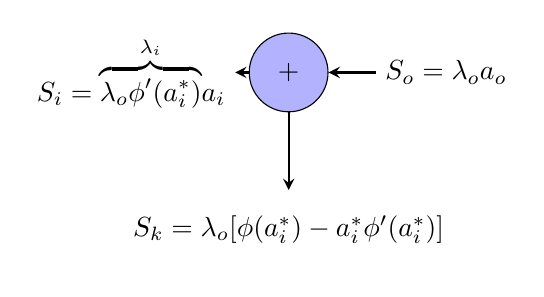
\begin{tikzpicture}[node distance=2cm]		
		\node (si) [startstop] {$S_i = \overset{\lambda_i}{\overbrace{\lambda_o \phi ' (a_i^*)}} a_i$};
		\node (score_calc) [process_score, right of=si] {$+$};
		\node (score_out) [startstop, right of=score_calc] {$S_o=\lambda_o a_o$};	
		\node (score_out_const)[startstop, below of=score_calc] {$S_k = \lambda_o [\phi(a_i^*) - a_i^* \phi ' (a_i^*)]$};
		
		\draw [arrow_back] (si) -- (score_calc);
		\draw [arrow_back] (score_calc) -- (score_out);	
		\draw [arrow] (score_calc) -- (score_out_const);	
		\end{tikzpicture}
		};
	\end{tikzpicture}
\end{document}

